\documentclass[a4paper,12pt]{article}           %   A4, pt changes regular font size
\frenchspacing                                  %   Finnish spacing
\usepackage{a4wide}                             %   Less margis
\usepackage[british]{babel}                     %   Edit this to match your language, e.g., finnish
\usepackage{xcolor}                             %   color support
    \definecolor{my_grey}{HTML}{7F7F7F}
\usepackage{icomma}                             %   Better comma in eqs. if used
\usepackage{hyperref}                           %   Clickable URLs
\usepackage{booktabs}                           %   Better tables
\usepackage{siunitx}                            %   Physics unit stuff
\usepackage{listings}                           %   Better tables
\usepackage{graphicx}                           %   Figures work
\usepackage{fontspec}                           %   Better way to handle custom fonts
\usepackage{amsmath}                            %   Basic math
\usepackage{esint}                              %   Various fancy integral symbols
\usepackage[capitalise]{cleveref}               %   \cref better than \ref
    \crefname{section}{Sec.}{Secs.}             %   Add abbreviation for Sections
\usepackage[position=top]{subfig}
    \captionsetup[subfigure]{position=top, labelfont=bf,textfont=normalfont,singlelinecheck=off,justification=raggedright}
\captionsetup[subfigure]{subrefformat=simple,labelformat=simple,listofformat=subsimple}
\renewcommand\thesubfigure{(\alph{subfigure})}
\usepackage{sectsty}                            %   Edit section titles
    %\allsectionsfont{\normalfont\sffamily}     %   ALL titles use sans-serif
    \sectionfont{\normalfont\sffamily\large\color{my_grey}} 
    \subsectionfont{\normalfont\sffamily\normalsize\color{my_grey}} 
    \subsubsectionfont{\normalfont\sffamily\small\color{my_grey}}
\setsansfont{URW Gothic L}[
    Path = fonts/,
    Extension =.ttf,
    UprightFont = * Regular,
    ItalicFont = * Italic,
    BoldFont = * Bold,
    BoldItalicFont= * Bold Italic]
\setmonofont{Source Code Pro}[
    Path = fonts/,
    Extension =.ttf,
    UprightFont = *-Regular,
    ItalicFont = *-Italic,
    BoldFont = *-Bold,
    BoldItalicFont= *-BoldItalic
]
\setmainfont{AdobeTextPro}[
    Scale = 0.958,
    Path = fonts/,
    Extension =.ttf,
    UprightFont = *-Regular,
    ItalicFont = *-It,
    BoldFont = *-Bold,
    BoldItalicFont= *-BoldIt]
\usepackage[libertine]{newtxmath}               %   Matching math font
\usepackage{fancyhdr}                           %   Nice header and footer header (and/or footer)
    \pagestyle{fancy}                               %   Makes package work
\usepackage[section]{placeins}                  %   Figures stay in declared section
\usepackage{minted}                             %   Beautiful verbatim code
    \usemintedstyle{emacs}                          %   code style
    \setminted{
        frame=lines,
        framesep=2mm,
        baselinestretch=0.9,
        fontsize=\footnotesize,
        linenos,
        breaklines
    }
\usepackage{csquotes}                           %   Correct quotes for babel
\usepackage[backend=biber,
            style=ieee,
            urldate=long,
            maxnames=5,
            dateabbrev=false]{biblatex}         %   Citation style with biblatex
\DeclareSourcemap{                              %   No ISSN for journals
    \maps[datatype=bibtex]{
        \map{
        \step[fieldset=issn, null]
        }
    }
}
\renewbibmacro*{doi+eprint+url}{                %   Print URL iff no doi
    \printfield{doi}
    \newunit\newblock{}
    \iftoggle{bbx:eprint}{
        \usebibmacro{eprint}
    }{}
    \newunit\newblock{}
    \iffieldundef{doi}{
        \usebibmacro{url+urldate}}
        {}
}

\hypersetup{
    pdfauthor={Niko Savola},                    %   Author here
}

\linespread{1.1}
\setlength{\headheight}{15pt}                   %   Suppress height warnings
\addtolength{\topmargin}{-2.4pt}


% Set commonly used math commands here
\newcommand*{\pd}[3][]{\ensuremath{\frac{\partial^{#1} #2}{\partial #3}}}
\newcommand*{\dt}[3][]{\ensuremath{\frac{\textrm{d}^{#1} #2}{\textrm{d} #3}}}
\newcommand{\dbar}{\textrm{d}\hspace*{-0.08em}\bar{}\hspace*{0.1em}}
\newcommand{\de}{\textrm{d}}
\newcommand{\sref}[1]{\textbf{\small\subref{#1}}}
\newcommand{\ve}[1]{\textbf{#1}}
\newcommand{\e}{\mathrm{e}}

\addbibresource{references.bib}
\hypersetup{
    pdftitle={Machine learning with many-body tensor networks | Niko Savola},
}
%   header
\lhead{\textsf{Special exercise}}
\chead{\textsf{PHYS-E0421 - Solid-State Physics}}
\rhead{\textsf{Niko Savola \textbf{653732}}}
%   footer
\lfoot{}
\cfoot{}
\rfoot{\thepage}


\usepackage[braket, qm]{qcircuit}  % Qiskit output

% \setminted{fontsize=\footnotesize, baselinestretch=1}

\begin{document}

\begin{titlepage}
    {\sffamily
    \noindent
    \fontsize{12}{14}\selectfont
    Aalto University \newline
    School of Science \newline
    Department of Applied Physics

    \vspace{40mm}

    \noindent
    \fontsize{14}{16}\selectfont
    \emph{Niko Savola}

    \vspace{10mm}

    \noindent
    \fontsize{18}{22}\selectfont
    \textbf{Machine learning with many-body tensor networks}\\

    \fontsize{12}{14}\selectfont
    \noindent
    Submitted for approval: \today

    \vspace{70mm}

    \noindent
    Special exercise \\[4mm]
    PHYS-E0421 \textendash{} Solid-State Physics \\[4mm]
    } % end of \sffamily

\end{titlepage}
\newpage


\section{Introduction}

Tensor networks have been originally developed for efficiently storing and manipulating high-dimensional quantum many-body states~\cite{PhysRevLett.69.2863}. These variational families of wavefunctions emerge from low-entanglement representations of quantum states. Contemporary applications however include a wide range of fields, such as, machine learning~\cite{Roberts2019}, statistical mechanics~\cite{Levin_2007}, quantum chemistry~\cite{White1999}, and cosmology~\cite{Bao_2017}.
This exercise aims to present the theory behind tensor networks and their use in machine learning. Then we present a numerical example for training a tensor network representing a quantum circuit, effectively pre-training a quantum computer for solving a problem.

% can be used in 


% TODO review paragraph.
% https://youtu.be/q8UTwdjS95k


\section{Theory}

\subsection{Tensor networks}

Tensor networks are a powerful tool for splitting a high-dimensional function into constituent parts of smaller tensors. 
Here a tensor refers to a multidimensional array, rank zero corresponding to a scalar, rank one to a vector, rank two to a matrix, and further ranks being referred to as rank $n$ tensors.

It is natural to use Tensor network notation (TNN), which can be considered a graphical generalisation of Einstein summation, for presenting Tensor networks~\cite{Bridgeman_2017}. This notation maps tensors to  nodes with lines corresponding to the rank of the tensor. The lines represent indices for the multidimensional array, see \cref{sfig:tensor_basics}.

The elegance of TNN arises from contracting tensors. Multiplication is done by linking the lines of the tensors. For example, matrix-vector multiplication consists of linking a node with one line to a node with two lines. The ensuing tensor will have one free line, resulting in a vector as expected.
This logic is further demonstrated for a few examples in \cref{sfig:tensor_samples}.
Notice how multiplication of high-rank tensors is rendered graphically trivial. This is indeed useful for representing complex architectures of tensor networks.



\begin{figure}[htb]
    \centering
    \subfloat[]{{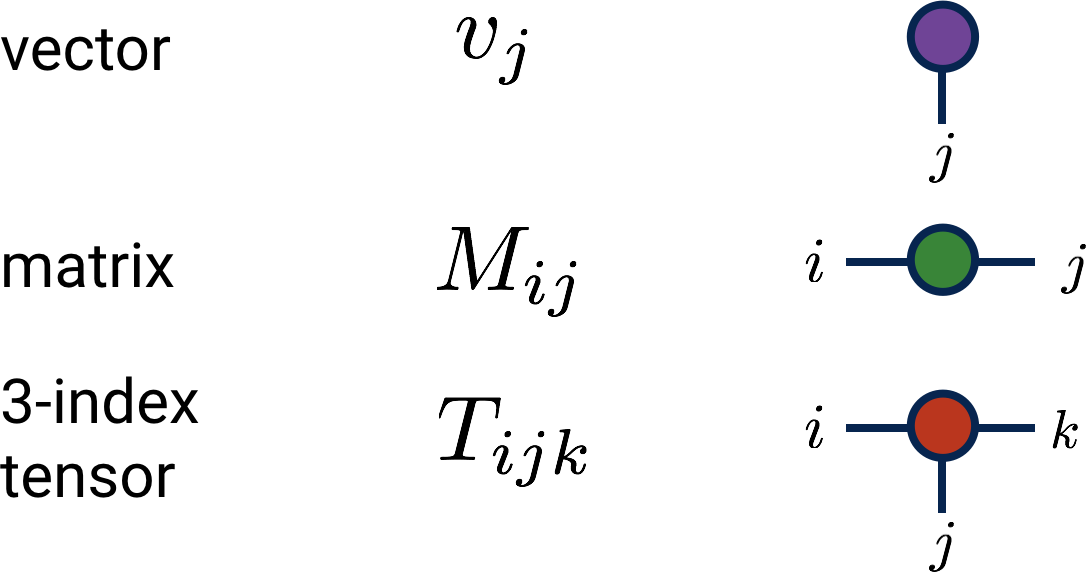
\includegraphics[width=0.43\textwidth]{figures/tensor_diagrams.png}\label{sfig:tensor_basics}}} \qquad
    \subfloat[]{{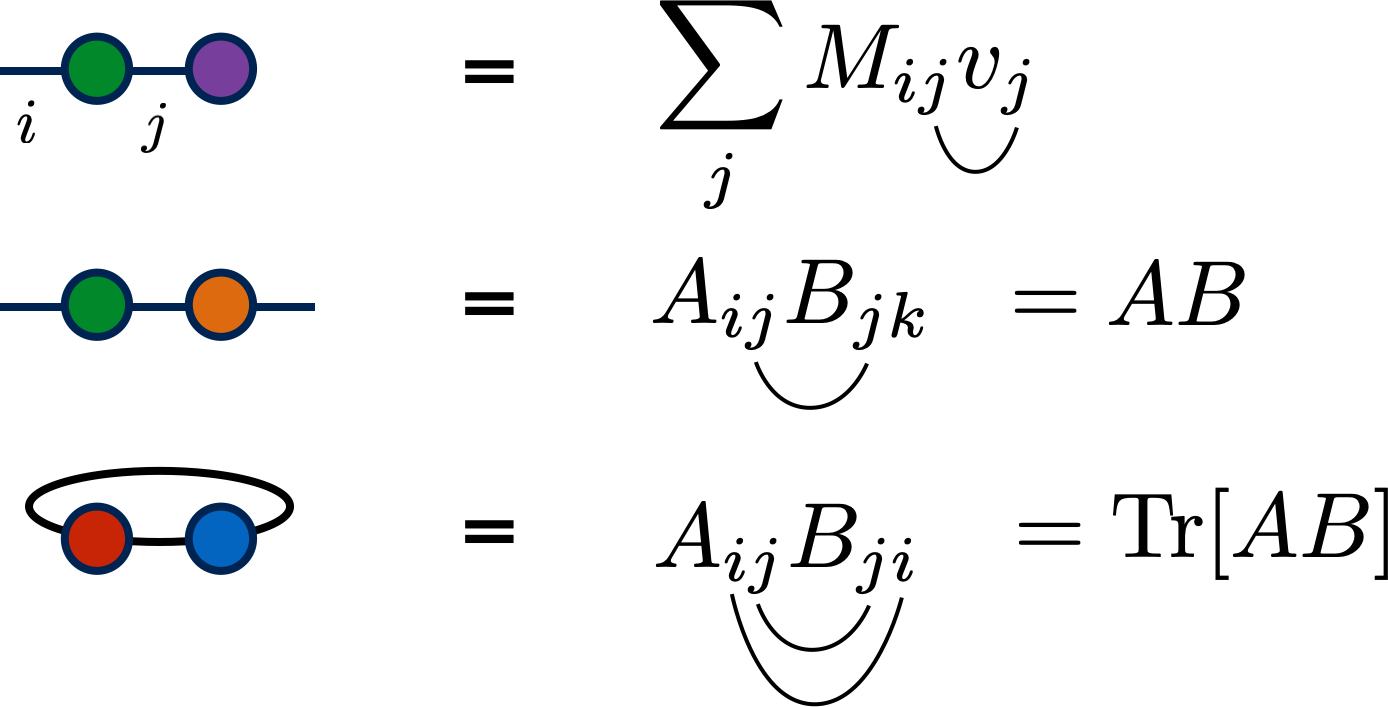
\includegraphics[width=0.45\textwidth]{figures/sample_contractions.png}\label{sfig:tensor_samples}}}
    
    \caption{\protect\subref{sfig:tensor_basics} Examples of low-rank tensors and their TNN representations. \protect\subref{sfig:tensor_samples} Examples of tensor contractions for matrices. From top to bottom: matrix-vector product, matrix multiplication, and their trace. Note how the last example elegantly results in a scalar. Schematics from Ref.~\cite{Stoudenmire2021}}
    \label{fig:tensor_diagrams}
\end{figure}

% TODO notation from https://arxiv.org/pdf/1905.01330.pdf


\subsubsection{Machine learning}

As interest in deep learning has skyrocketed~\cite{DL_review}, using Tensor networks in conjunction with neural networks (NN) has been explored.
Although tensor networks are still an active research topic, some prominent tensor network architectures for machine learning have emerged, such as, Matrix Product States (MPS) and Tensor Renormalization Group (TRG).

TODO MPS


TODO TRG https://tensornetwork.org/trg/


One branch of research involves using a tensor network directly as machine learning model architecture. Another uses tensor networks to compress layers in neural network architectures or for other auxilary tasks.

a paradigm called differentiable programming.

TODO MPS


In fact, it has been shown that there exists a mapping from generative neural networks referred to as Restricted Boltzmann machines to Tensor networks~\cite{PhysRevB.97.085104}, highlighting the link to deep learning.


\subsection{Modelling many-body physics}

todo work as Ansätze


\section{Numerical implementation}


% https://quimb.readthedocs.io/en/latest/examples/ex_tn_train_circuit.html


\cite{Roberts2019}


\begin{minted}{python}
# the hamiltonian
H = qu.ham_ising(n, jz=1.0, bx=0.7, cyclic=False)
\end{minted}



\section{Example: Training a quantum circuit for unitary evolution}

todo


\begin{figure}[htb]
    \centering

    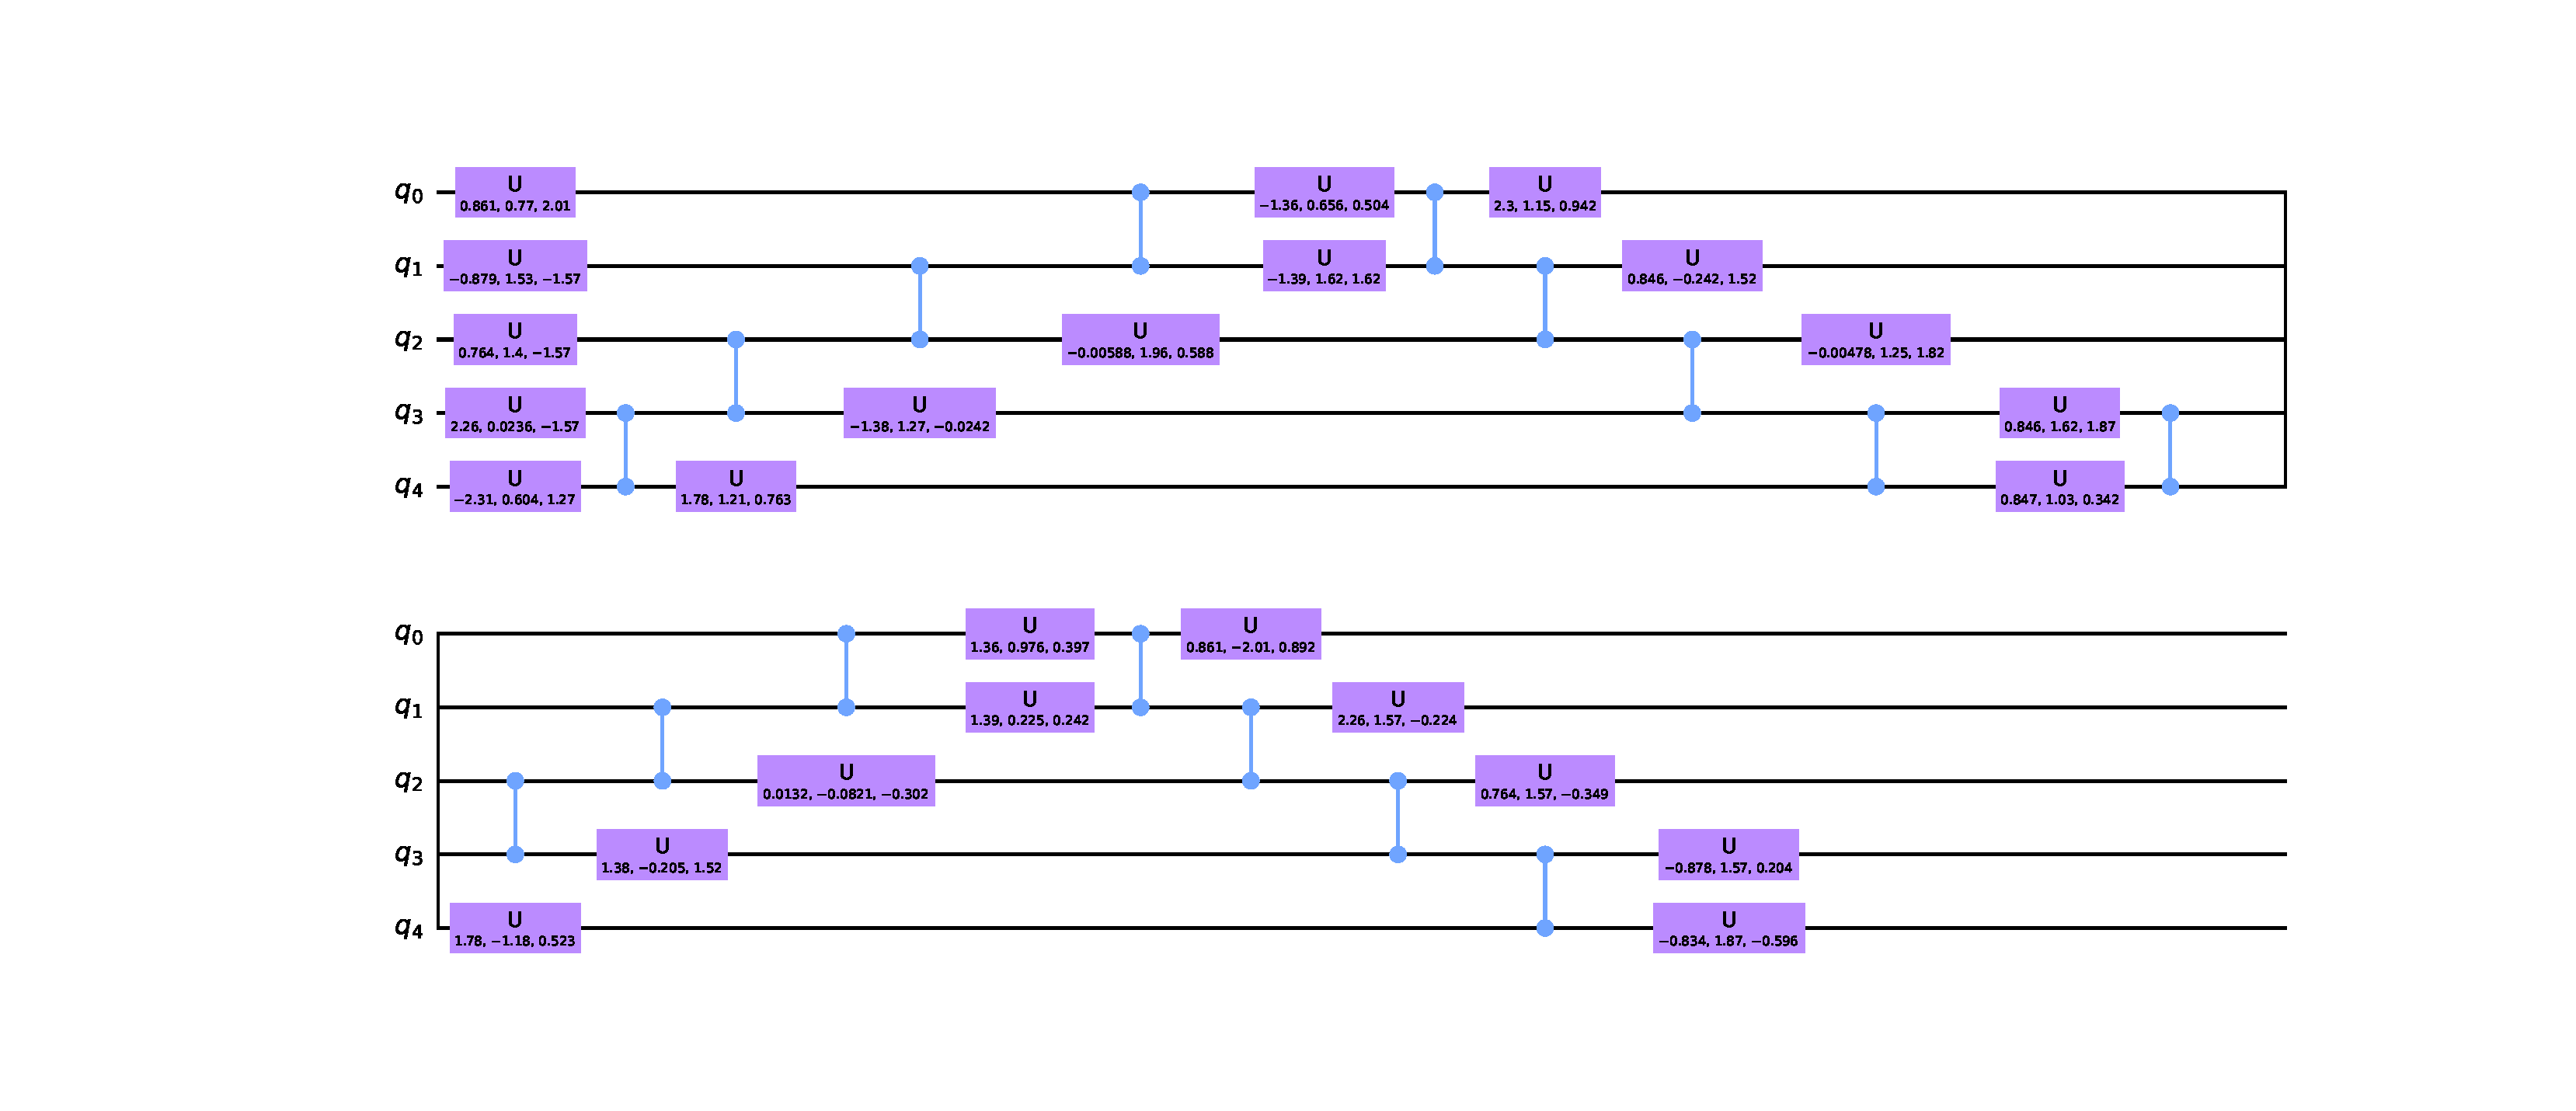
\includegraphics[width=0.97\textwidth]{figures/ansatz_circuit.pdf}

    \caption{<caption>}
    \label{fig:qasm_circuit}
\end{figure}



todo suprajohto qubit toteutus
https://arxiv.org/pdf/2103.12305.pdf




but the motivation is that the architecture generalises to unknown problem

\section{Summary}

Todo





TODO https://github.com/google/TensorNetwork

https://arxiv.org/pdf/1905.01331.pdf

%-------------------
%   Bibliography
%-------------------

\newpage
\pagestyle{plain}
%\setlength\bibitemsep{1.3\itemsep}
%\setlength\bibitemsep{0.1\baselineskip}
\addcontentsline{toc}{section}{Viitteet}
\renewcommand*{\bibfont}{\footnotesize}
\printbibliography{}


\end{document}
